% !TEX root = ../main.tex
% fix page break in toc
% \addtocontents{toc}{\protect\newpage}
\chapter{Results}
  %
  % ========
  \section{Identical particles correlations}
  % ========
    %
    % ========
    \subsection{Spherical harmonics components}
    % ========
      \begin{figure}[h]
        \centering
        \centerline{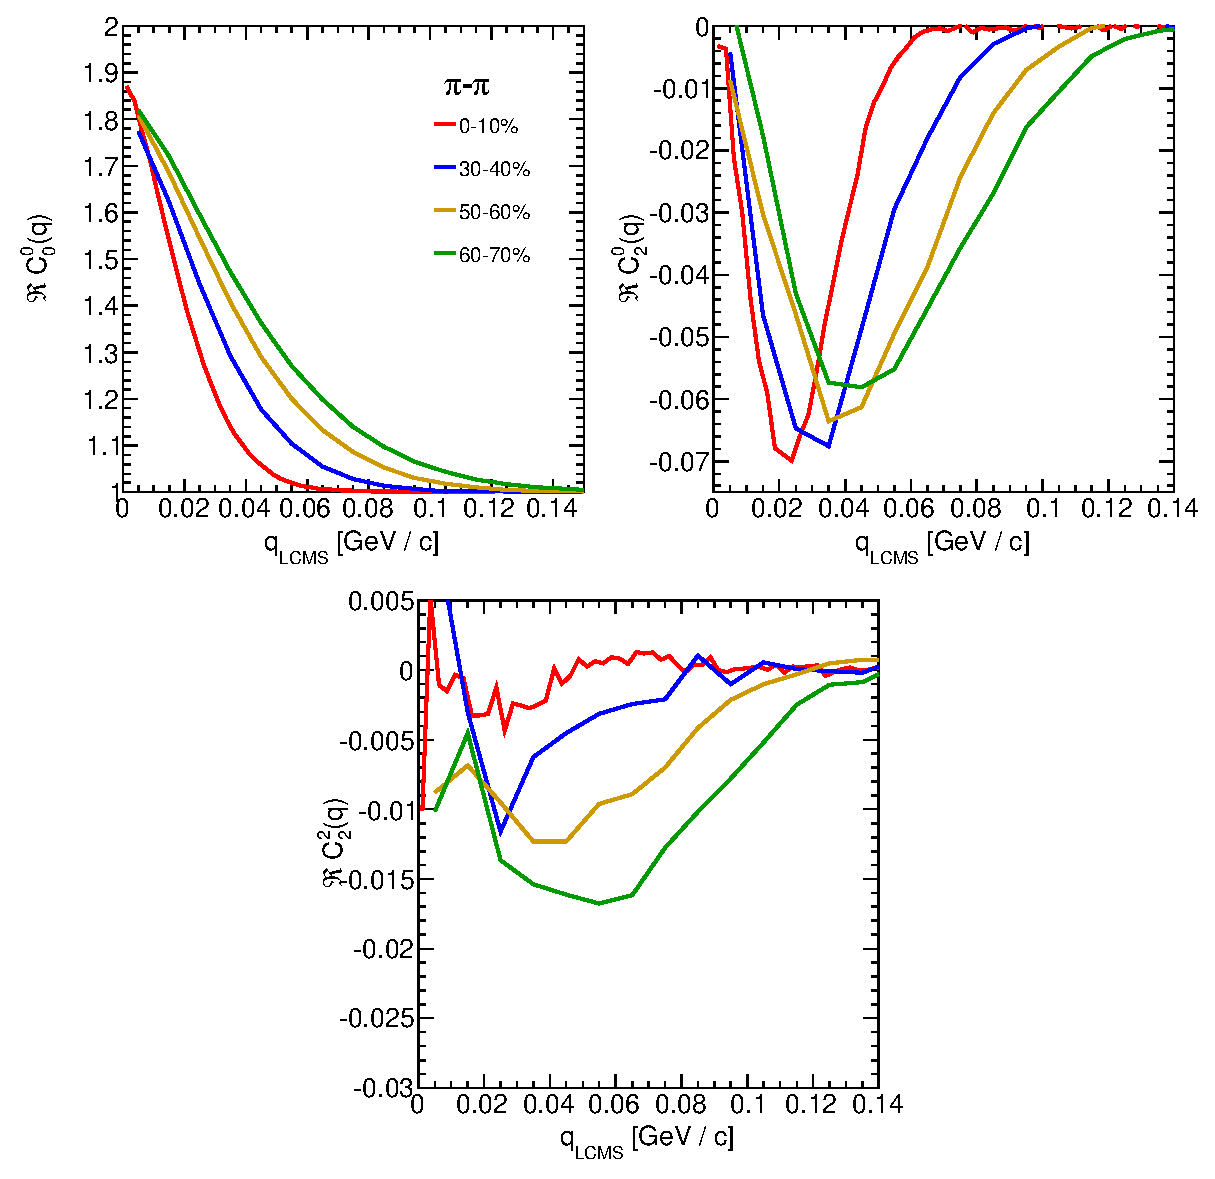
\includegraphics[width=1.0\textwidth]{results/cf3dpi}}
        \caption{no caption}
      \label{fig:cf3dpi}
      \end{figure}

      \begin{figure}[h]
        \centering
        \centerline{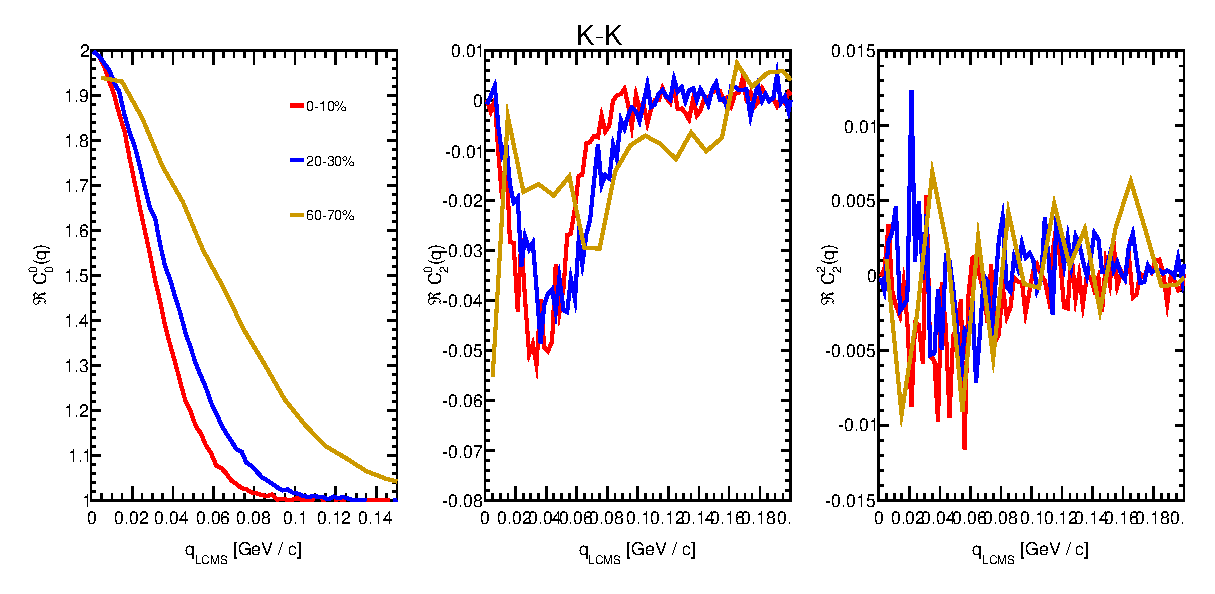
\includegraphics[width=1.0\textwidth]{results/cf3dk}}
        \caption{no caption}
      \label{fig:cf3dk}
      \end{figure} 

      \begin{figure}[h]
        \centering
        \centerline{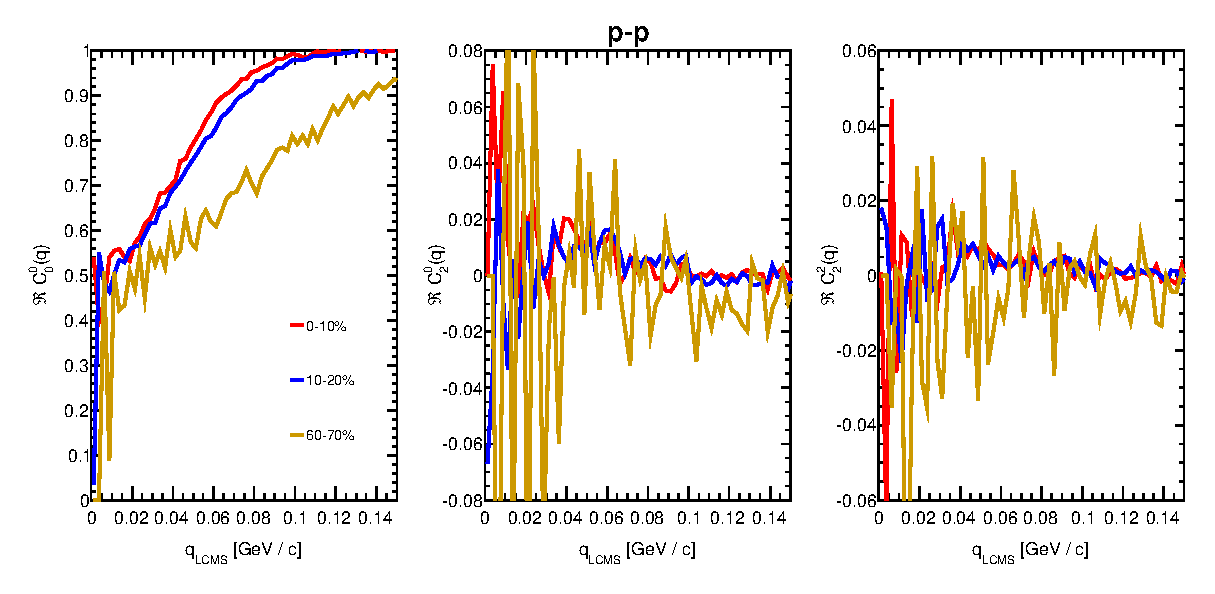
\includegraphics[width=1.0\textwidth]{results/cf3dp}}
        \caption{no caption}
      \label{fig:cf3dp}
      \end{figure}  
    \FloatBarrier
    %
    % ========
    \subsection{Centrality dependence of a correlation function}
    % ========
    % napisac o singletowym bozonow i trypletowym protonow
    % pokazac poszerzenie CF vs k_T oraz vs centralnosc
      \begin{figure}[h]
        \centering
        \centerline{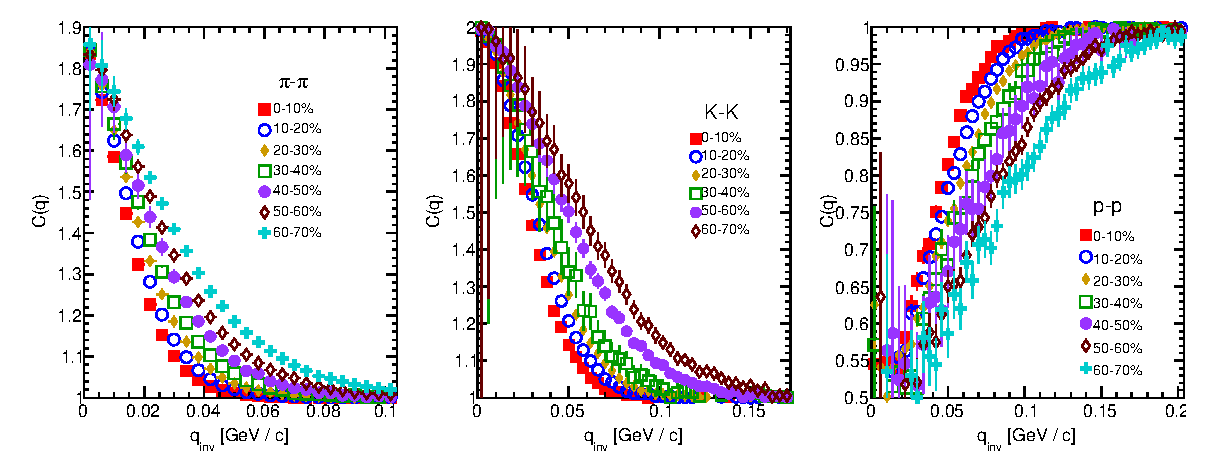
\includegraphics[width=1.0\textwidth]{results/cfvsctr}}
        \caption{no caption}
      \label{fig:centr_dep}
      \end{figure}
    \FloatBarrier
    %
    % ========
    \subsection{$k_T$ dependence of a correlation function}
    % ========
      \begin{figure}[h]
        \centering
        \centerline{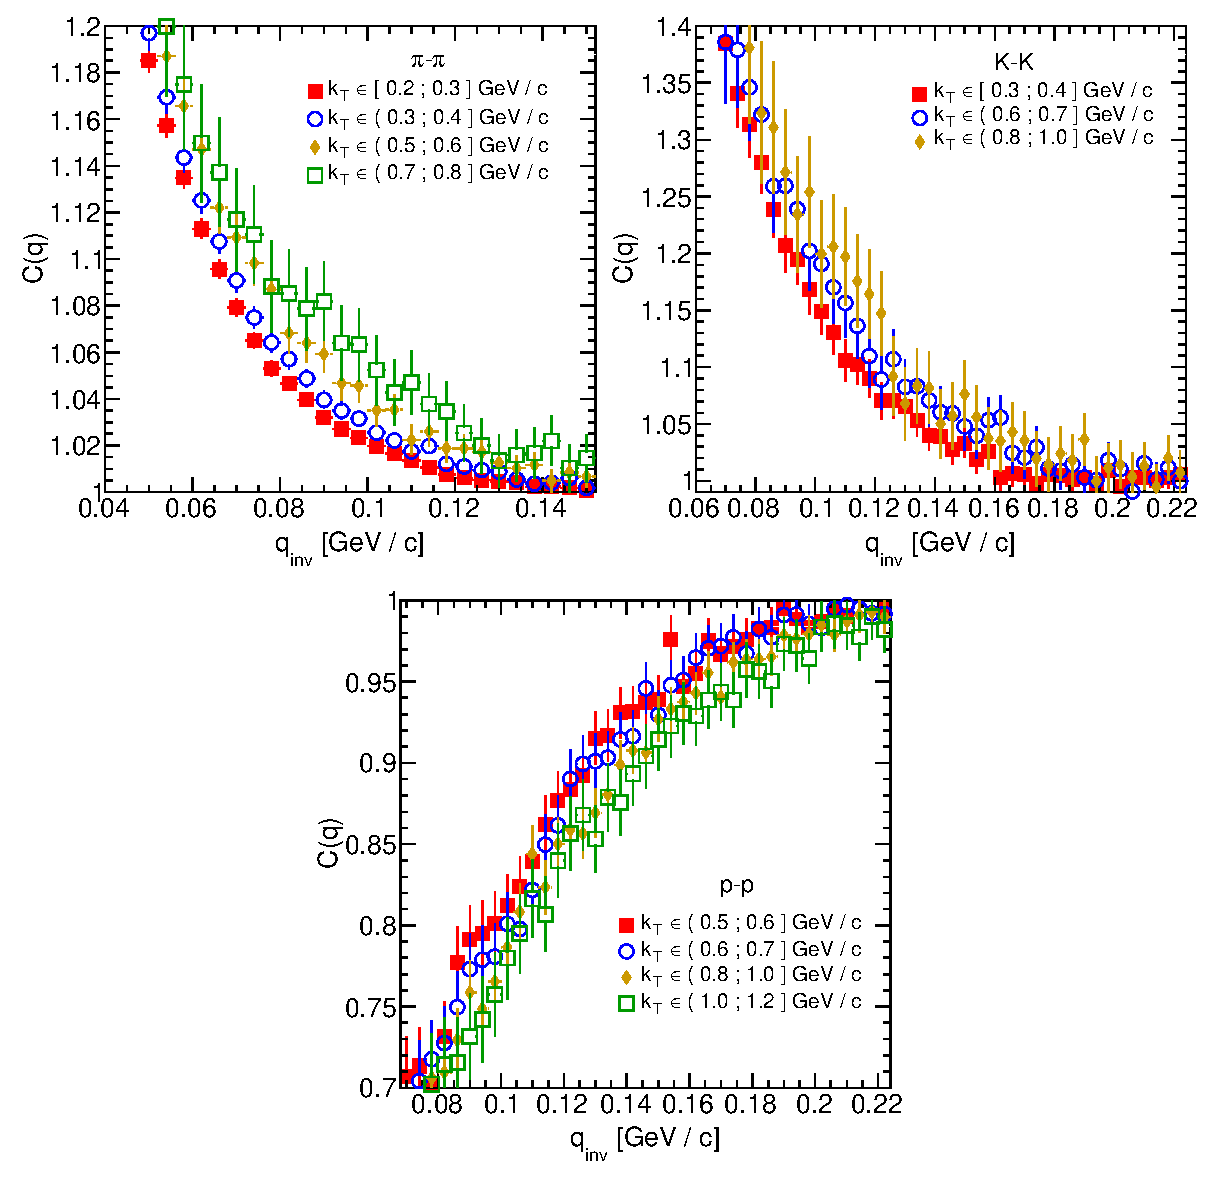
\includegraphics[width=1.0\textwidth]{results/cfvskt}}
        \caption{no caption}
      \label{fig:kt_dep}
      \end{figure}
    \FloatBarrier
  %
  % ========
  \section{Results of the fitting procedure}
  % ========
    %
    % ========
    \subsection{Femtoscopic radii scaling with the transverse mass}
    % ========
      \begin{figure}[h]
        \centering
        \centerline{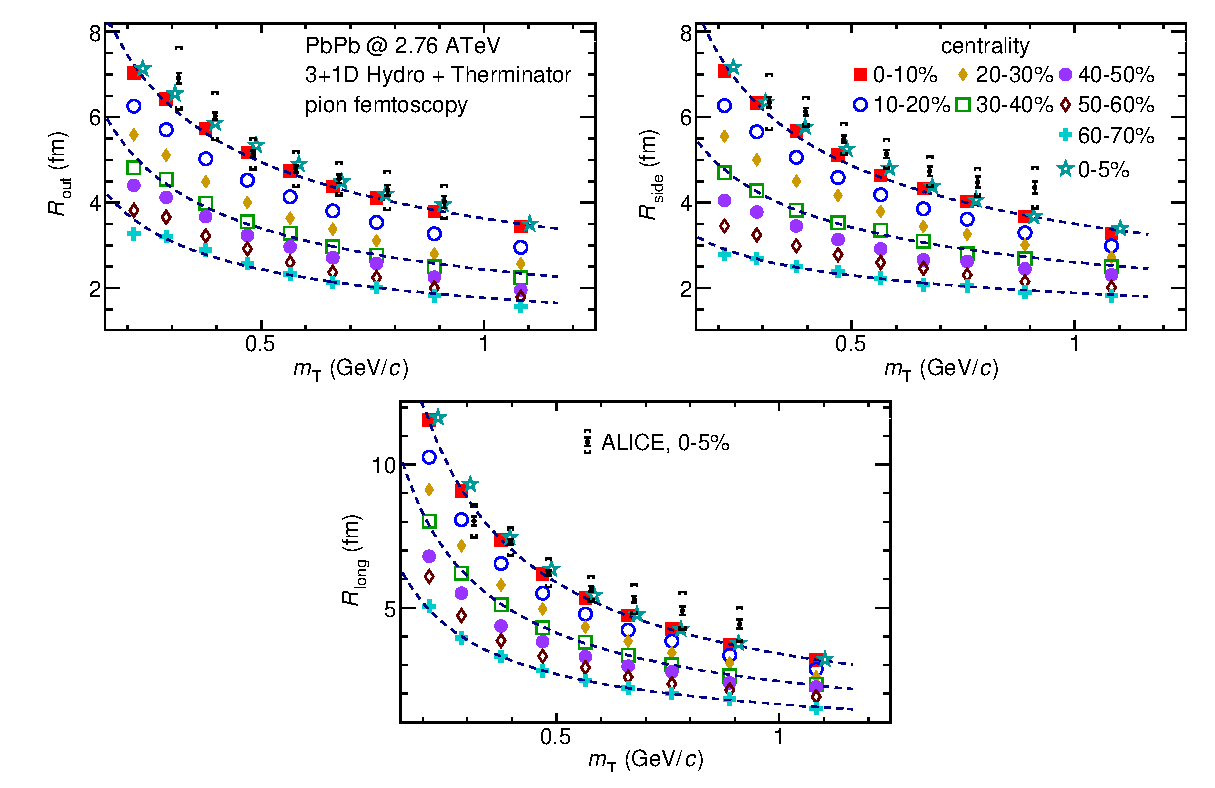
\includegraphics[width=1.05\textwidth]{results/piradii}}
        \caption{no caption~\cite{alice_pion}~\cite{galazyn}.}
      \label{fig:piradii}
      \end{figure}



      \begin{figure}[h]
        \centering
        \centerline{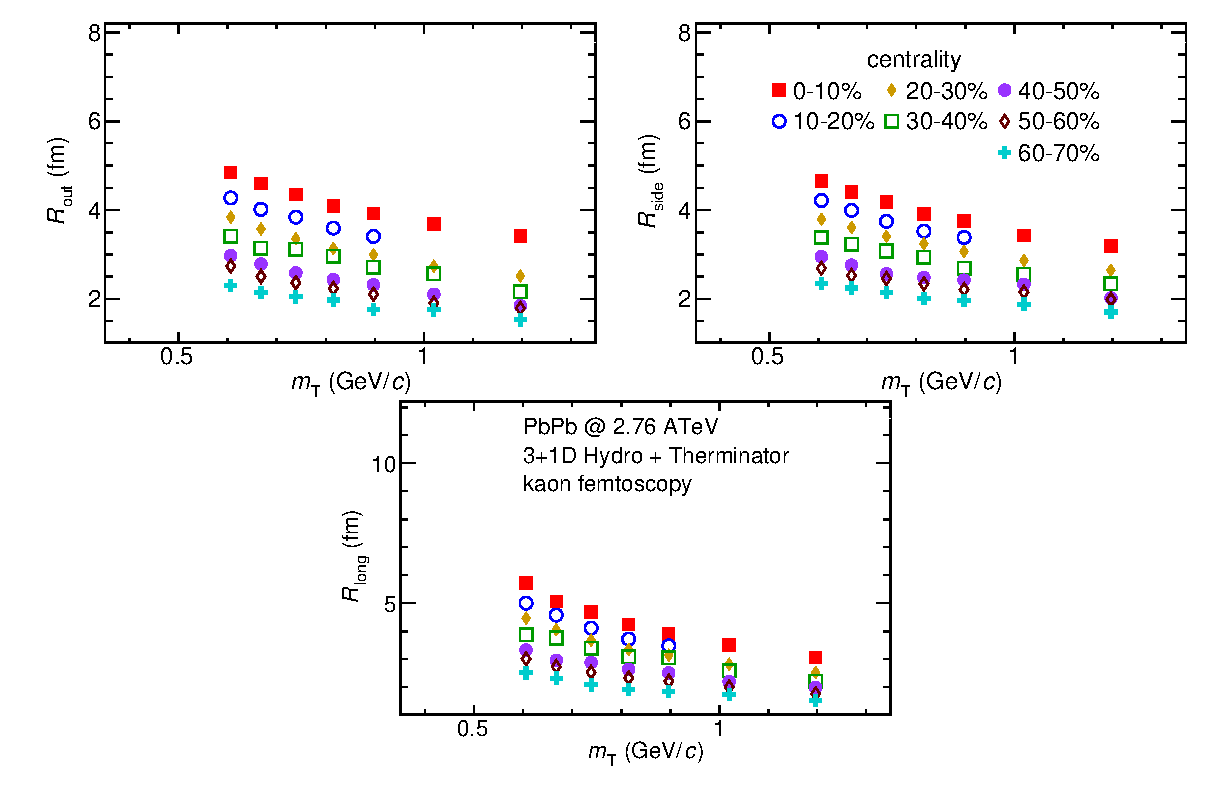
\includegraphics[width=1.05\textwidth]{results/kradii}}
        \caption{no caption~\cite{galazyn}.}
      \label{fig:kradii}
      \end{figure}



      \begin{figure}[h]
        \centering
        \centerline{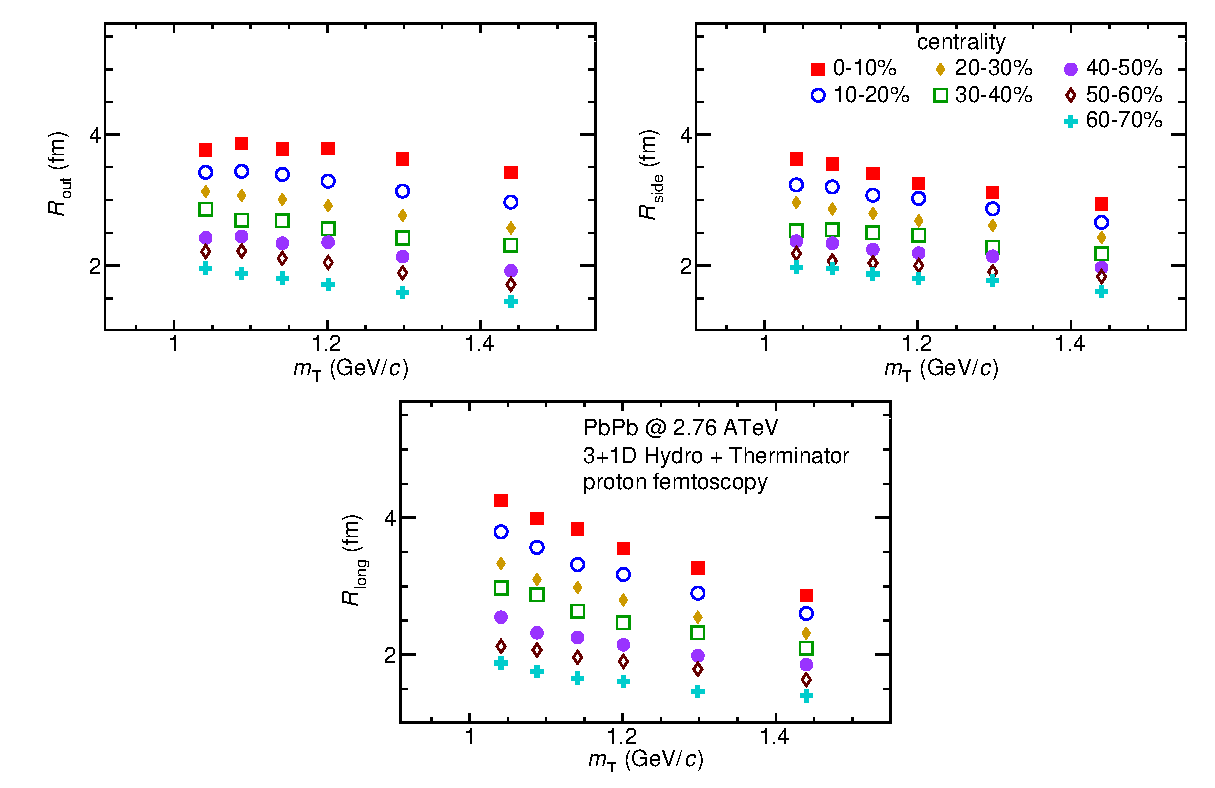
\includegraphics[width=1.05\textwidth]{results/pradii}}
        \caption{no caption~\cite{galazyn}.}
      \label{fig:pradii}
      \end{figure}    

      \begin{figure}[h]
        \centering
        \centerline{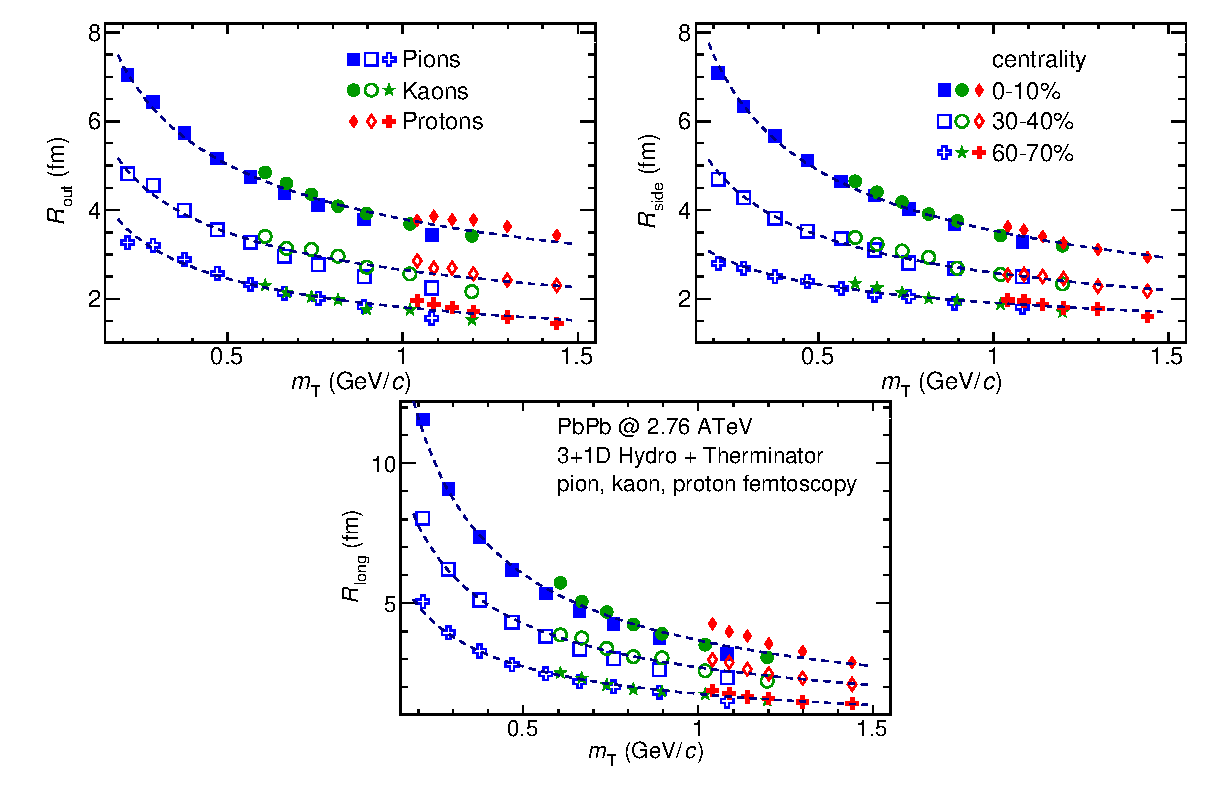
\includegraphics[width=1.05\textwidth]{results/allradii_lcms}}
        \caption{no caption~\cite{galazyn}.}
      \label{fig:allradii}
      \end{figure}    

      \begin{figure}[h]
        \centering
        \centerline{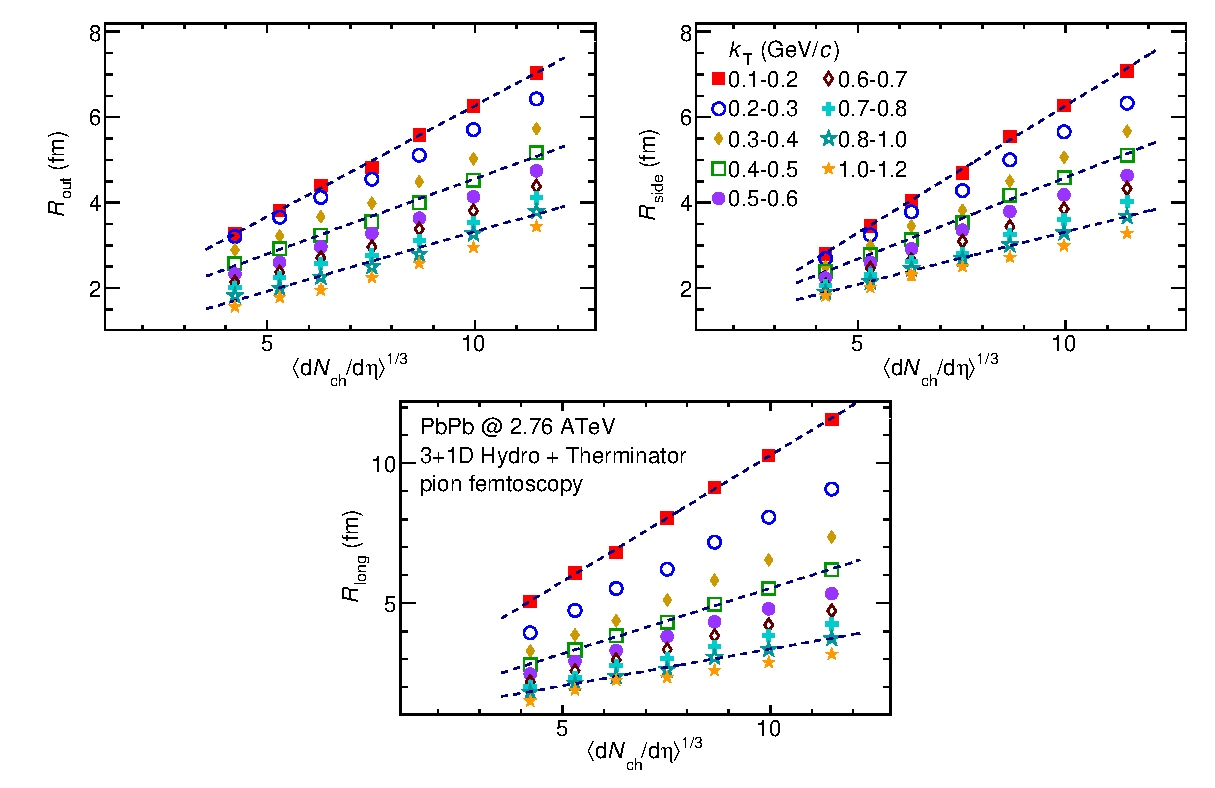
\includegraphics[width=1.05\textwidth]{results/piradii_vs_nch}}
        \caption{no caption~\cite{galazyn}.}
      \label{fig:piradii}
      \end{figure}    

      \begin{figure}[h]
        \centering
        \centerline{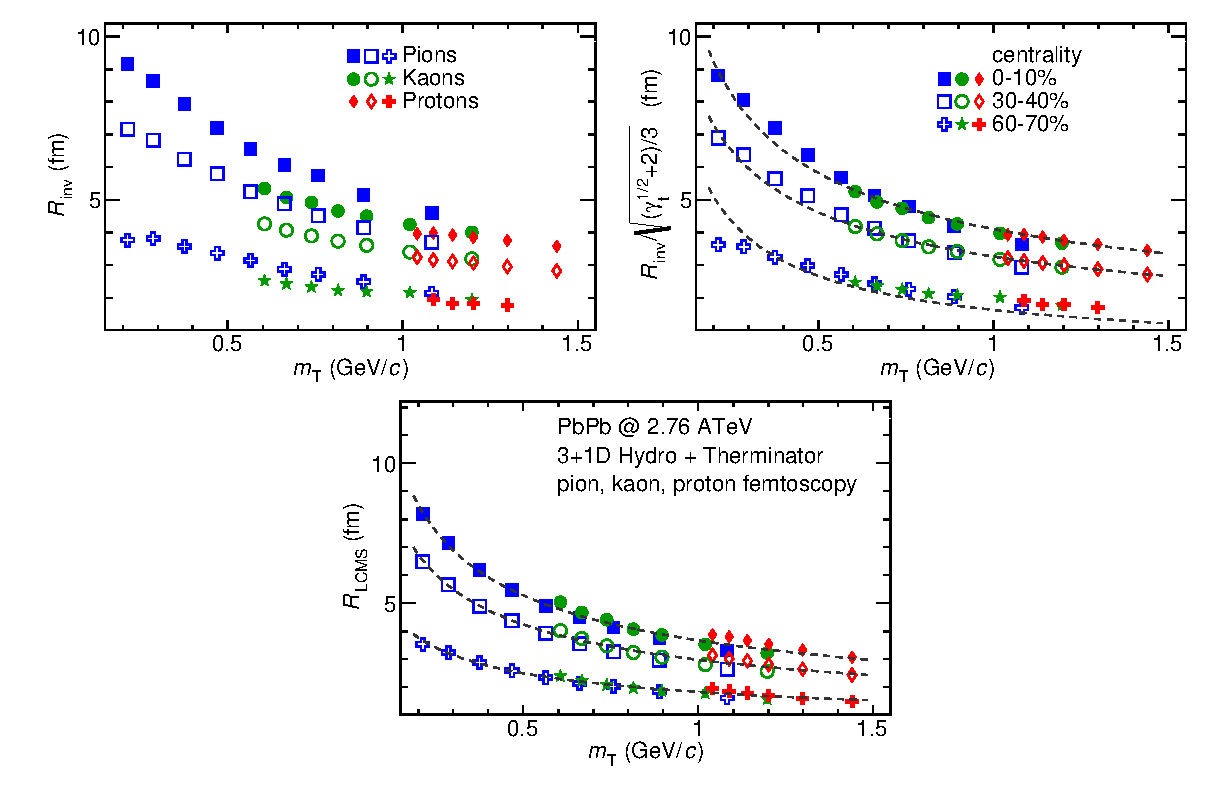
\includegraphics[width=1.05\textwidth]{results/scaling_test}}
        \caption{no caption~\cite{galazyn}.}
      \label{fig:piradii}
      \end{figure}    

      \begin{figure}[h]
        \centering
        \centerline{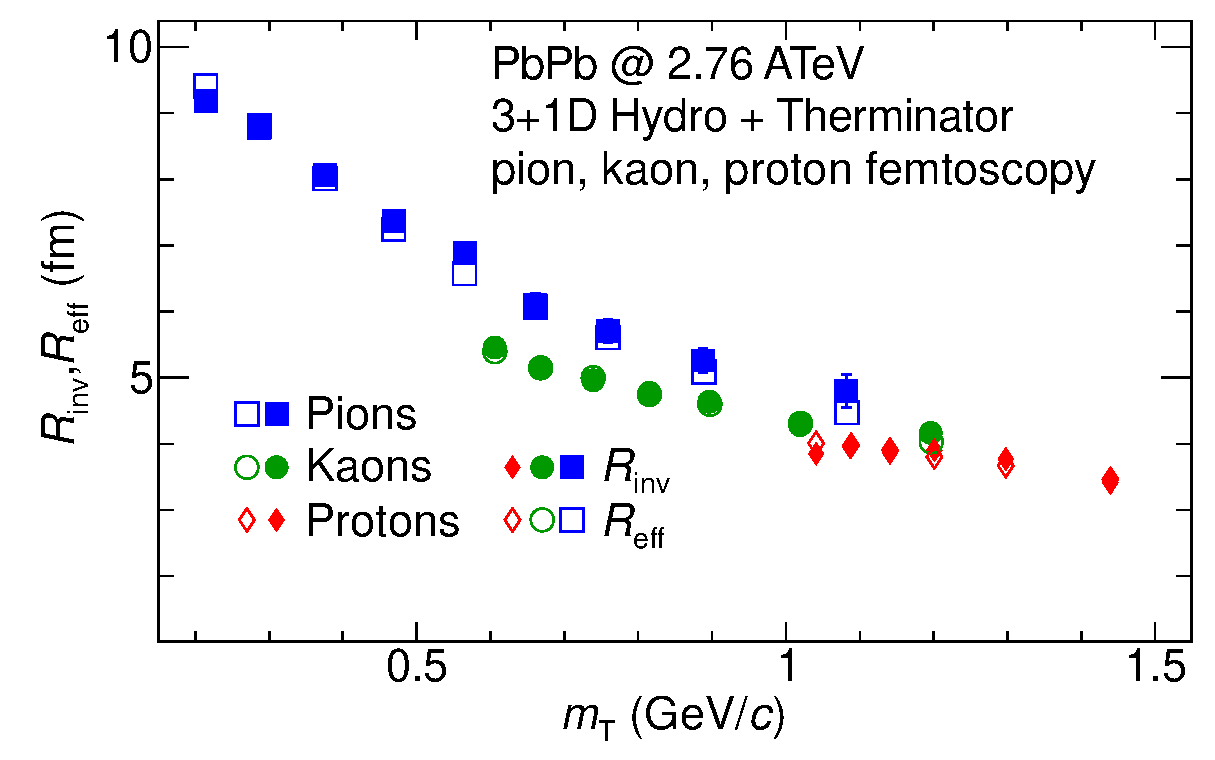
\includegraphics[width=0.55\textwidth]{results/rinvreff}}
        \caption{no caption~\cite{galazyn}.}
      \label{fig:piradii}
      \end{figure}

    \FloatBarrier
  %
  % ========
  \section{Discussion of results}
  % ========
